%-------------------------------------
% CONFIGURATION
%-------------------------------------

\documentclass[hidelinks,11pt]{article}

% TABLE PATHS
\makeatletter
\def\input@path{{./Shipping Emissions Paper includes/tables/}}
\makeatother

% JUSTIFICATION
\usepackage{geometry}
\geometry{
	paper=letterpaper, % Change to letterpaper for US letter
	top=2.5cm, % Top margin
	bottom=2.5cm, % Bottom margin
	left=2.5cm, % Left margin
	right=2.5cm, % Right margin
	%showframe, % Uncomment to show how the type block is set on the page
}
\usepackage{microtype} % Improve justification
\usepackage[onehalfspacing]{setspace}

% % SECTIONS, REFERENCES, AND CITATIONS
\usepackage[hyperfootnotes=false]{hyperref}
\hypersetup{
    colorlinks=false, %links not colored
    linktoc=all %link to both section and subsections
}
\usepackage[english]{babel}
\addto\extrasenglish{
	\def% -------------------------------------------------
\sectionautorefname{Section}
  \def\subsectionautorefname{Section}
	\def\subsubsectionautorefname{Section}
}
\usepackage[backend=biber,style=apa,autocite=inline,hyperref=false]{biblatex} 
\usepackage{csquotes}
\DeclareLanguageMapping{english}{english-apa}
\addbibresource{shippingemissionstrade.bib}
% Use shortauthor when available
\makeatletter
\AtEveryCitekey{\ifnameundef{shortauthor}{}{\def\cbx@apa@ifnamesaved{\@firstoftwo}}}
\makeatother

\usepackage[nolist,nohyperlinks]{acronym}

\usepackage[compact]{titlesec}
%% The following commands causes chapter and section references to
%% uppercase the part name.
\renewcommand{\chapterautorefname}{Chapter}
\renewcommand{\sectionautorefname}{Section}
\renewcommand{\subsectionautorefname}{Section}
\renewcommand{\subsubsectionautorefname}{Section}

% MATH FORMATTING
\usepackage{amsmath}
\usepackage{mathtools}
\usepackage{amssymb}

% GRAPHICS
\usepackage{graphicx} % Allows including images
\graphicspath{{./Shipping Emissions Paper includes/plots/}}
\usepackage{float} % Allows for control of float positions

% TABLE FORMATTING
\usepackage[table]{xcolor} % for color in tables
\usepackage{booktabs}
\usepackage{multirow}
\usepackage{makecell}
\renewcommand\theadalign{cc}
\renewcommand\theadfont{\bfseries}
\renewcommand\theadgape{\Gape[1pt]}
\renewcommand\cellalign{cl}
\renewcommand\cellgape{\Gape[1pt]}
\usepackage{threeparttable} % regression notes on tables
\usepackage{adjustbox} % adjust table width

% % GENERAL
\usepackage{enumerate}

% TITLE PAGE

\title{Improving Maritime Shipping Emissions Estimates Using Machine Learning}

\date{\today}

%---------------------------------------
% DOCUMENT
%---------------------------------------

\begin{document}

\begin{titlepage}

\maketitle

\begin{abstract}
    We employ machine learning to improve upon engineering estimates of \acl{CO2} emissions from maritime shipping. Traditional estimates rely on engineering approximations that may not entirely capture actual fuel use. We match reported annual ship-level emissions from a \acl{EU} emissions reporting program with tracking data and technical characteristics for the global fleet of dry bulk ships. Following industry standard procedures, we calculate engineering estimates of annual ship-level emissions and include these values as a predictor. We train various machine learning algorithms on reported fuel consumption and achieve high out-of-sample prediction accuracy.
	% - emphasize performance over calc (in abstract)
	% - three data sets
\end{abstract}


% % \vfill
% % \textit{Keywords:} 
% % \textit{JEL codes: }
% % \textit{JEL codes (2-digit): }

\thispagestyle{empty} % Removes page number from first page
\end{titlepage}

%% The following is a directive for TeXShop to indicate the main file
%%!TEX root = diss.tex

% \chapter{Glossary}

% This glossary uses the handy \latexpackage{acroynym} package to automatically
% maintain the glossary.  It uses the package's \texttt{printonlyused}
% option to include only those acronyms explicitly referenced in the
% \LaTeX\ source.  To change how the acronyms are rendered, change the
% \verb+\acsfont+ definition in \verb+diss.tex+.

% use \acrodef to define an acronym, but no listing
% \acrodef{UI}{user interface}
\acrodef{UBC}{University of British Columbia}
\acrodef{FC}{fuel consumption}

% The acronym environment will typeset only those acronyms that were
% *actually used* in the course of the document

% search for potential acronyms using \s[A-Z]{2,}\s
% {
% \renewcommand{\baselineskip}{0em}
% \begin{acronym}
% \setlength{\parskip}{0ex}
% \setlength{\itemsep}{0ex}
\acrodef{IMO}[IMO]{International Maritime Organization}
\acrodef{IPCC}[IPPC]{Intergovernmental Panel on Climate Change}
\acrodef{UNCTAD}[UNCTAD]{United Nations Conference on Trade and Development}
\acrodef{CO2}[CO$_2$]{carbon dioxide}
\acrodef{MRV}[MRV]{Monitoring, Reporting, and Validation}
\acrodef{EU}[EU]{European Union}
\acrodef{AIS}[AIS]{Automatic Identification System}
\acrodef{GDP}[GDP]{gross domestic product}
\acrodef{OECD}[OECD]{Organisation for Economic Co-operation and Development}
\acrodef{DWT}[DWT]{tons deadweight}
\acrodef{RMSE}[RMSE]{root-mean-squared error}
\acrodef{WIP}[WIP]{world industrial production}
\acrodef{USD}[USD]{United States dollars}
\acrodef{GHG}[GHG]{greenhouse gas}
\acrodef{MAPE}[MAPE]{mean absolute percentage error}
\acrodef{MAE}[MAE]{mean absolute error}
\acrodef{MSE}[MSE]{mean squared error}
\acrodef{HFO}[HFO]{heavy fuel oil}
\acrodef{OLS}[OLS]{ordinary least squares}
\acrodef{R2}[R$^2$]{coefficient of determination}
\acrodef{nm}[nm]{nautical miles}
\acrodef{GT}[GT]{gross tonnage}
\acrodef{WFR}[WFR]{World Fleet Register}
\acrodef{MMSI}[MMSI]{Maritime Mobile Service Identity}
\acrodef{ME}[ME]{main engine}
\acrodef{AE}[AE]{auxiliary engine}
\acrodef{BO}[BO]{boiler}
\acrodef{TPC}[TPC]{tonnage per centimeter}
\acrodef{NT}[NT]{net tonnage}
\acrodef{t}[t]{tonnes}
% \end{acronym}
% }

% You can also use \newacro{}{} to only define acronyms
% but without explictly creating a glossary
% 
% \newacro{ANOVA}[ANOVA]{Analysis of Variance\acroextra{, a set of
%   statistical techniques to identify sources of variability between groups.}}
% \newacro{API}[API]{application programming interface}
% \newacro{GOMS}[GOMS]{Goals, Operators, Methods, and Selection\acroextra{,
%   a framework for usability analysis.}}
% \newacro{TLX}[TLX]{Task Load Index\acroextra{, an instrument for gauging
%   the subjective mental workload experienced by a human in performing
%   a task.}}
% \newacro{UI}[UI]{user interface}
% \newacro{UML}[UML]{Unified Modelling Language}
% \newacro{W3C}[W3C]{World Wide Web Consortium}
% \newacro{XML}[XML]{Extensible Markup Language}

\section{Introduction}\label{MLintro}

% Motivation:
% - Shipping emissions are a significant contributor to global CO$_2$ emissions.
% - Traditional estimates rely on engineering approximations that may not entirely capture actual fuel use.
% - Higher frequency estimates (typically published with lag)
% - Existing estimates may suffer from poor data quality
The most recent official estimate of \ac{GHG} emissions from maritime shipping places the sector's contribution at around 3\% of global emissions \parencite{faber2020fourth}. Since this estimate was published, various events have significantly impacted the shipping industry, including the COVID-19 pandemic and the implementation of new measures aimed at improving ship efficiency. Such events have almost certainly had immediate effects on emissions, and quantifying their magnitude can provide insights into the effectiveness of actual policy measures and how to improve them. To do so, it is essential to have accurate and timely estimates of emissions. In this paper, we develop a prediction methodology that augments the industry-standard method based on engineering relationships with machine learning in order to provide more accurate estimates. These estimates can be updated and published in real-time, providing invaluable information for policymakers, researchers, and industry stakeholders alike.

% What we do:
% - Provide a machine learning approach to more accurately estimate CO$_2$ emissions
% - Higher frequency estimates (typically published with lag)
% - Take emissions reports as truthful and accurate
% - Predict fuel consumptions directly, providing bottom-up approach as predictor (perhaps a sort of featuring engineering)
% - Dealing with missing data for extrapolation
% - We are able to explain x\% of variation in residual
% - Better untracked (no AIS data) predictions???

To develop and evaluate our model of shipping emissions, we leverage publicly available emissions reporting data from the \ac{MRV} program implemented by the \ac{EU}. \Ac{CO2} emissions are directly proportional to fuel consumption,\footnote{For example the most common fuel, \ac{HFO}, emits 3.114 kg \ac{CO2} per kg of fuel.} and we therefore take (log) reported annual ship fuel consumption as our target variable. We evaluate various machine learning algorithms, using data on both ship characteristics and ship activity as predictor variables. Crucially, we include features derived from the engineering-based fuel consumption calculations used by the \ac{IMO}. These features use hourly ship activity observations from \ac{AIS} data, including location, speed, and draft,\footnote{Draft is the vertical distance between the waterline and the bottom of the hull. It is a function of how heavily laden the ship is and affects fuel consumption.} to construct annual aggregate features in a manner that is consistent with the physics that determine fuel use. This approach allows us to leverage physics-based formulas while also flexibly allowing for deviations from them due to factors that are unaccounted for or inaccurately measured.

Using our hybrid approach, we are able to achieve a high degree of accuracy in predicting fuel consumption. For our data set comprising the global fleet of dry bulk ships, our best-performing model achieves an out-of-sample \ac{R2} of 0.954 and \ac{MAPE} of 10.9\%.\footnote{Our training set consists of data from 2019 and 2020, and our hold-out test sample is 2021 data.} This is a significant improvement over a purely calculation-based approach, which achieves an \ac{R2} of 0.58 and an \ac{MAPE} of 20.4\%. We evaluate both linear models (\ac{OLS}, lasso, and ridge) and tree-based models (random forest, gradient boosting Regression, and CatBoost). While ridge regression performs the best in terms of \ac{R2} for our hold-out sample, we find that all models perform quite well, with even the worst-performing achieving an \ac{R2} of 0.931 (\ac{MAPE}=12.3\%).
% Value sources: ML_FC_Fm2_test_fc.csv, generated by ML_FC.ipynb

% Contribution and results preview:
% - Machine learning provides a flexible functional form that can:
%     - Capture divergence from engineering relationships
%     - Help to mitigate error from imperfect/incomplete tracking data
%     - predict based on speed (OECD does not!)
% - Bottom-up vs. top-down
%     - How do reported values compare?
%     - How do our estimates compare?

The primary contribution of this work is a highly accurate methodology for predicting fuel consumption that can be used to produce timely estimates of shipping emissions under varying ship activity, such as travel speed. To our knowledge, this is the first study to directly predict fuel consumption using a hybrid of the industry-standard bottom-up calculation method and machine learning and apply it at a large geographic scale. The closest work to ours is that of \textcite{yan2023analysis} and \textcite{clarke2023co2} who both apply machine learning models to predict a ship-level annual average \ac{CO2} emission ratio with units of mass-per-distance-travelled. They obtain total emissions by multiplying this efficiency metric by the observed or reported distance travelled. Employing this approach for prediction relies on the assumption that fuel efficiency ``averages out'' over various operating conditions (e.g., speed) during a year for which fuel consumption is reported. While this may provide a satisfactory approximation when ship speeds remain similar to those used to train the model, it is in general biased due to the nonlinearity of fuel consumption with speed. As such, the error may be large when attempting to predict emissions under scenarios in which ships adjust their speed of travel, for example in response to emissions regulations.

We propose an alternative prediction methodology that has the similar data requirements for prediction, but leverages engineering and physics relationships to improve prediction performance across a wider range of operating conditions. We construct a predictor variable representing annual ship-level energy use by summing theoretical hourly energy use, which is calculated with the industry-standard Admiralty formula \parencite[p.~64]{faber2020fourth}. This formula relies on ship characteristics and hourly speed and draft observations. To allow for potential inaccuracies in the functional form, we also construct slight variations on this quantity and provide these as additional predictor variables.

% Clarke 2023: "The emissions efficiency ratio variable average CO2 emissions per nautical mile from the EU-MRV dataset was chosen as the target variable for the random forest model due to having high coverage in the EU-MRV dataset, and the ability to adapt it according to distances travelled, a variable that we can obtain using the AIS. In addition, ratio indicators provide more stability than level indicators, for example total CO 2 emissions. In this case, efficiency as defined by emissions per distance travelled also benefits from ease of interpretation. The assumptions underpinning this approach are that the technical specifications of a vessel stay constant in the short term, that differences in emissions efficiency during a voyage average out, and that changes in a ship’s emissions come principally from the amount of distance covered in a given time period. In this way, we exploit ship characteristics to determine emission patterns, while using real-time movement
% information of the AIS dataset to calculate timely and frequent estimates of ships’ emissions. The random forest model departs from equation (1) above by learning emission patterns such that a ship’s full real-time development, including its engines’ status and operational mode as provided by AIS, do not need to be
% explicitly modelled. This approach builds on a similar strategy used by team Blue Carbon from the Wärtsilä Corporation25 in the 2020 UN Hackathon for AIS data."


%  Why does this work better?
%  reduces demand on machine learning model to capture physics of fuel consumption
%  potential inaccuracies in formulas
%  potential data errors that we can condition on
Our methodology balances the advantages of both calculation-based and pure machine learning approaches. Compared to other machine learning approaches, our use of engineering- and physics-based relations to engineer predictor features means we rely less on the machine learning algorithms to capture the physics of ship fuel consumption. The fact that linear models (in logs) perform similarly to non-linear, tree-based models in our analysis is consistent with this conjecture. In contrast to a purely calculation-based approach, incorporating machine learning allows the model to capture deviations from theoretical relationships, as well as incorporate further information that may have predictive power, but for which there is no theoretical foundation to suggest a functional form. One example of this is our inclusion of additional features derived from \ac{AIS} tracking data that provide information on both ship behaviour and potential data errors, which is a well-known issue researchers face when using this data.

% Literature:
% - Bottom-up approach
%     - IMO Fourth GHG Study \parencite{faber2020fourth}
% - Bottom-up approach + MRV data
% - Shipping Emissions and Machine Learning
%     - OECD \cite{clarke2023co2}

This paper is related to three strands of literature. The first of these has developed various bottom-up emissions estimation methodologies using engineering calculations applied to \ac{AIS} tracking data (e.g., \cite{jalkanen2009modelling,olmer2017greenhouse,moreno2019comparative,tvete2020modelling}). We build directly from these techniques in constructing our predictor variables. In particular, we follow the methodology used in the most recent \ac{IMO} emissions report as closely as possible \parencite{faber2020fourth}. A second strand of literature has begun to utilize annual emissions reports from the \ac{EU}'s \ac{MRV} program to validate emissions estimates obtained with the bottom-up approach. The largest study in scope is the \ac{IMO}'s analysis, however only the first year of \ac{MRV} reporting was available at the time \parencite{faber2020fourth}. Subsequently, a handful of authors have provided similar analyses, albeit with very limited geographical scope (e.g., \cite{doundoulakis2022comparative,mannarini2020eu,hensel2020green,wu2023evaluation}). In contrast, we analyse emissions from all dry bulk ships entering the \ac{EU}, and provide a methodology for global estimates. Furthermore, rather than using the \ac{MRV} data to simply validate predictions, we employ it to improve upon previous estimation methodologies. Lastly, a recent strand of literature applies various machine learning techniques to improve shipping emissions estimates. The majority of these use high-frequency fuel consumption data, but focus on small geographic areas and/or numbers of ships (e.g. \cite{ren2022container,wang2023ship,hu2019prediction,jebsen2020estimating,monisha2023step}). \textcite{guo2022combined} use machine learning primarily to model the physics of weather effects on ship resistance in a computationally feasible manner, thereby extending the application of previous calculation-based model from \textcite{tvete2020modelling}. Our work employs readily available annual fuel consumption data, which allows us to study emissions on a much larger scale. As described above, our work is similar in objective to that of \textcite{yan2023analysis} who employ gradient boosting and \textcite{clarke2023co2}, who use random forest regression to predict ship-level fuel \textit{efficiencies}. We directly predict fuel consumption, which allows us to leverage predictors derived from engineering calculations, and thereby obtain very high prediction accuracy for fuel consumption and emissions.

\section{Data}\label{sec:MLdata}
We obtain data on the global fleet of dry bulk ships, which includes annual fuel consumption reports, hourly tracking data, and ship characteristics, jointly spanning the years 2019 to 2021. 

Since 2018, fuel consumption reports are publicly available from the \ac{EU} \ac{MRV} program, which requires commercial ships over 5,000 \ac{GT} to report their total annual fuel consumption and distance travelled for all voyages into and out of the European Economic Area (henceforth referred to as EU trips) \parencite{eu2015regulation}. We take the reported annual fuel consumption, in \ac{t}, for \ac{EU} trips as ground truth,\footnote{The \ac{MRV} program requires third-party validation of all reports to ensure accuracy. Furthermore, during the period that we study there were no binding emissions regulations and therefore no clear incentive to misreport fuel consumption.} and take the log to construct our target variable. 
% TODO: Mention average and sd at least, maybe plot
% TODO: plot histogram of FC for all bulk vs. matched?

Ship characteristics are taken from the \ac{WFR}, purchased from Clarksons Research, which includes a wide range of ship characteristics, such as ship type, size, engine power, etc. We match these characteristics to the \ac{EU} \ac{MRV} data using the \ac{IMO} number, a unique identifier for each ship. We retain only dry bulk carriers, after which between 3,600 and 3,900 ship observations remain per year, comprising roughly 30\% of the global dry bulk fleet.\footnote{We consider dry bulk to include all ships over 10,000 \acs{DWT} categorized in the \acs{WFR} under Ore Carrier, Bulk Carrier, Chip Carrier, Open Hatch Carrier, Forest Product Carrier, Aggregates Carrier, Cement Carrier, Nickel Carrier, and Slurry Carrier.}
% Value sources: ML_preprocessing.py

% TODO: Check for representativeness in appendix?

Ship tracking data consists of messages transmitted by \aclp{AIS} (\acs{AIS}) fitted to each ship, which rely on global positioning systems and radio transmitters to track and report the ship's activity. Our dataset is purchased from Spire and contains hourly transmissions from all dry bulk ships, recorded by both land- and satellite-based receivers. Draft observations from static \ac{AIS} messages are merged to dynamic messages by hour and \ac{MMSI}, which identifies a ship's transceiver. Draft values are input manually by the ship's crew and therefore many observations are missing. We follow a commonly-used strategy and replace each missing draft value with the last valid observation.
% TODO: quantify missing draft values in appendix and reference here

\ac{AIS} data is subject to various sources of error, and we largely follow standard procedures to clean it, which are described in greater detail in \autoref{app:ML}. We employ an intentionally conservative cleaning strategy, and rely on a final validation step with the \ac{MRV} (described at the end of this section) to ensure that valid data is used to train our model. Throughout, we employ the haversine formula to calculate distances between location observations in an accurate and computationally feasible manner.

One common error we observe are physically infeasible changes in a ship's trajectory and/or location. Since many of these are single, anomalous observations, we first drop single data points that represent an abrupt change of direction that is infeasible for the speed at which the ship is travelling. In other cases, a ship (as identified by the \ac{MMSI}), appears to jump to a new location, pursue a feasible trajectory for some time, and then jump back to its previous location. To correct for this type of error, we split each ship's trajectory whenever both the distance between observations exceeds 140 \ac{nm} and the implied speed (calculated as distance divided by time between observations) exceeds 25 knots. We retain either the even or odd trajectory segments depending on which set comprises the greater number of observations. The resulting data set contains trajectories for 12,716 unique \ac{MMSI}.
% Source: AIS_Calculations.py
% TODO: add and reference summary stats in appendix for:
% - jumps
% - ships with multiple segments
% - dropped points
% - how many span full three years?

A second important error is missing dynamic data, i.e. hours for which there is no observation for a ship. We interpolate these missing data points as per the \ac{IMO}'s strategy \parencite{faber2020fourth}, creating an observation for each missing hour, assuming a constant speed and using the haversine formula to interpolate location coordinates. Speed is interpolated as the distance between consecutive locations divided by the time difference, and the previous draft value is assigned. On average, 37\% of observations for each ship-year are interpolated, although this figure varies widely, with a standard deviation of 21\%. This average decreases year-on-year, from 46\% in 2019 to 30\% in 2021. 
% Source: AIS_Calculations_Interp.py

To match the cleaned \ac{AIS} tracking data to the \ac{MRV} reports, it is necessary to identify which observations to attribute to \ac{EU} trips, as only activity related to those trips is reported in the \ac{MRV} data. To do so, we first identify port calls based on observed speed and proximity to land.\footnote{We identify a port call when a ship does not exceed a speed of one knot for at least 12 hours and is within a nation's economic exclusion zone (200 \ac{nm} from the coast).}\footnote{This strategy will tend to detect more than the correct number of port calls, as these are defined in the regulation as occurring only when cargo is loaded or unloaded, however this is not directly observable from the tracking data \parencite{eu2015regulation}.} A trip is defined as a ship's movement between two port calls. As per the \ac{EU} \ac{MRV} regulation, any trip with at least one of its two port calls within the jurisdiction of an \ac{EU} member state is considered an \ac{EU} trip \parencite{eu2015regulation}.\footnote{Ports in the United Kingdom ceased to be included as of the beginning of 2021.} To obtain the various annual values we use as predictors (see \autoref{sec:MLmethodology}), we aggregate over all observations assigned to an \ac{EU} trip in each year. These annual aggregate values are then matched to the \ac{MRV} and \ac{WFR} data by \ac{MMSI} and year. We successfully match 1989 ships for 2019, 2084 for 2020, and 2349 for 2021.
% Source: ML_preprocessing.py
% TODO: more detail in appendix?

Finally, given the potential for errors stemming from the raw \ac{AIS} data and the trip detection procedure, we develop our model using a subset of data for which the observed distance travelled on EU trips agrees well with the reported distance. Specifically, we select only those ship-year observations for which the calculated and reported distances agree within 500 \ac{nm}.\footnote{As a robustness check, we also apply an alternative criterion of $\pm$10\%.} Summary statistics of the resulting data set are provided in \autoref{tab:reportstats}. We pool the observations from 2019 and 2020 to construct a training set of 1281 observations, while the observations from 2021 are set aside for out-of-sample testing.
% Source: ML_prepocessing.py

\begin{table}
    \centering
    % \begin{adjustbox}{max width=\textwidth}
    \begin{threeparttable}
        \caption{Reported fuel consumption summary statistics}
        \label{tab:reportstats}
        
\begin{tabular}[t]{>{\centering\arraybackslash}p{4em}>{\raggedleft\arraybackslash}p{3em}>{\raggedleft\arraybackslash}p{3em}>{\raggedleft\arraybackslash}p{3em}}
\toprule
\multicolumn{1}{>{\centering\arraybackslash}p{4em}}{Year} & \multicolumn{1}{>{\centering\arraybackslash}p{3em}}{count} & \multicolumn{1}{>{\centering\arraybackslash}p{3em}}{mean} & \multicolumn{1}{>{\centering\arraybackslash}p{3em}}{sd}\\
\midrule
2019 & 585 & 1389 & 932\\
2020 & 671 & 1311 & 951\\
2021 & 692 & 1334 & 932\\
\bottomrule
\end{tabular}

        % \begin{tablenotes}[flushleft]\small
            % \item \textit{Note:} MAE is mean absolute error, and $R^2$ is the coefficient of determination. The best score for each metric is highlighted in bold.
        % \end{tablenotes}
    \end{threeparttable}
    % \end{adjustbox}
\end{table}

% TODO: add some plots of summary stats to demonstrate representativeness of retained data
% TODO: Compare to page 140 of IMO Fourth GHG Study [@faber2020fourth]


\section{Methodology}\label{sec:MLmethodology}

We train a model of fuel consumption in two steps: First, we calculate theoretical annual fuel consumption based on the bottom-up methodology used by the \ac{IMO}. Second, we train machine learning models to predict fuel consumption, using as predictors both the calculated fuel consumption and additional ship characteristics. We evaluate the performance of these models using a cross-validation procedure with the training data as well as on a separate test set.

\subsection{Engineering Calculation}\label{subsec:engcalc}
% Generally following the IMO Fourth GHG Study
We follow closely the \ac{IMO} procedure described in \textcite{faber2020fourth} to calculate theoretical fuel consumption, with only a few minor simplifications. The key steps are outlined below, and further details are provided in \autoref{app:ML}. 

A ship's total instantaneous fuel consumption, $FC_{i}$, is the sum of the fuel consumed by each of the \acf{ME}, \acf{AE}, and \acf{BO}, each of which is the product of the demanded power $W_{i}$ and the specific fuel consumption $SFC_{i}$ for that component:
% Admiralty formula, other
\begin{equation*}
    FC_{i} = W_{\text{ME},i} \cdot SFC_{\text{ME},i} + W_{\text{AE},i} \cdot SFC_{\text{AE},i} + W_{\text{BO},i} \cdot SFC_{\text{BO},i}.
\end{equation*}

Demanded power is the power required to move the ship through the water (and air). For the \acl{AE} and \acl{BO}, power values are assigned based on the ship's operating phase, as determined by its speed and distance from shore. For the \acl{ME}, demanded power is given by the Admiralty formula, which is nonlinear in speed $v$ and draft $t$:
% TODO: phase assignment in appendix

\begin{equation}\label{eqn:admiralty}
    W_{\text{ME},i} = C \cdot W_{\text{ME},\textit{ref}} \cdot \left( \frac{t_i}{t_{\textit{ref}}} \right)^{0.66} \cdot \left( \frac{v_i}{v_{\textit{ref}}} \right)^{3},
\end{equation}

where $C$ is a constant applied to correct for factors such as weather and hull fouling, and the \textit{ref} subscript denotes reference values that are maximum ratings taken from ship specifications in the \ac{WFR}.
% TODO: detail static values in appendix (or data section?)

Specific fuel consumption describes the efficiency of each engine. For the \acl{AE} and \acl{BO} this is taken to be constant and equal to $SFC_{base}$, while efficiency of the \acl{ME} is taken to be quadratic in engine load (the ratio of demanded power to reference power):

\begin{equation*}
SFC_{\text{ME},i} = SFC_{\text{base}} \cdot \left(0.455 \cdot \left(\frac{W_{\text{ME},i}}{W_{\text{ME},\textit{ref}}}\right)^2 - 0.710 \cdot \frac{W_{\text{ME},i}}{W_{\text{ME},\textit{ref}}} + 1.280\right).
\end{equation*}

$SFC_{\text{base}}$ is assigned based on the ship's engine type, fuel type, and year built.
% TODO: SFC_base in appendix
% (see \autoref{app:ML})

% SFC_base
%   - Phase assignment

To aggregate, we assume operating conditions are constant over each hour (the frequency of the interpolated observational data) so that hourly fuel consumption is simply obtained by multiplying by the duration of each observation, $t$, equal to one hour. Annual fuel consumption $FC$ is then the sum over all observations $j$ in a year:

\begin{equation}\label{eqn:annual_fc}
    FC = \sum_j FC_{i,j} \cdot t.
\end{equation}

% Instantaneous values of draft, speed, and location taken from hourly \ac{AIS} data clearly aggregate non-linearly via the above equations.

\subsection{Machine Learning}\label{subsec:machinelearning}
% Intro - which models we consider
We evaluate the performance of several machine learning algorithms, both linear and tree-based. These include linear regression, lasso, ridge regression, gradient boosting regression, random forest regression, and CatBoost.\footnote{We use Python's Scikit-learn library for all but CatBoost, for which we use the CatBoost library.}
% Why not NN?

We consider as predictor variables both ship characteristics from the \ac{WFR} and activity-dependent variables derived from \ac{AIS} tracking data. Given the hundreds of characteristics available and the potentially infinite variations on aggregating tracking data, we select a set of features based on a combination of domain knowledge and feature importance results from preliminary analyses. These are described in \autoref{tab:features}. The features we derive from tracking data can be split into three categories. The first includes straightforward aggregation of observational behaviour, such as total distance travelled, number of trips taken, and fraction of time spent at ports. The second category includes the fuel consumption calculated as per \autoref{subsec:engcalc}, as well as components of the Admiralty formula \eqref{eqn:admiralty}. Lastly, we include variables that represent aspects of the quality of the tracking data, including the number of interpolated observations when the ship is at sea (when most fuel is consumed) and the longest distance between observations.

\begin{table}
    \centering
    \begin{adjustbox}{max width=\textwidth}
    \begin{threeparttable}
        \caption{Variable definitions}
        \label{tab:features}
        
\begin{tabular}[t]{>{\raggedright\arraybackslash}p{16em}>{\raggedright\arraybackslash}p{30em}}
\toprule
Variable & Description\\
\midrule
\addlinespace[0.3em]
\multicolumn{2}{l}{\textbf{Ship Characteristics}}\\
\hspace{1em}Age & Age at observation (years)\\
\hspace{1em}Beam Moulded & Maximum width (meters)\\
\hspace{1em}Deadweight Tonnage & Capacity (tonnes)\\
\hspace{1em}Draft & Maximum draft (meters)\\
\hspace{1em}Length Between Perpendiculars & Length between the forward and aft perpendiculars (meters)\\
\hspace{1em}Length Overall & Total length (meters)\\
\hspace{1em}Main Engine Power & Power rating of main engine (kilowatts)\\
\hspace{1em}Net Tonnage & Dimensionless index based on the total volume of cargo spaces\\
\hspace{1em}Size Category & e.g., Handymax, Panamax, etc.\\
\hspace{1em}Speed & Representative speed from \ac{WFR} (service or average observed) (knots)\\
\hspace{1em}Tonnage Per Centimeter & Load change required to change draft by one centimeter (tonnes/cm)\\
\addlinespace[0.3em]
\multicolumn{2}{l}{\textbf{Ship Activity}}\\
\hspace{1em}At-Port Fraction & Fraction of hourly observations with operational phase ‘at-port’\\
\hspace{1em}Distance Travelled & Distance calculated from AIS data (nautical miles)\\
\hspace{1em}Number Of Trips & Number of trips detected from AIS data\\
\addlinespace[0.3em]
\multicolumn{2}{l}{\textbf{Calculated}}\\
\hspace{1em}Admiralty Draft Term & Aggregation of draft term of (\ref{eqn:admiralty}), calculated as $\sum (t/t_{\textit{ref}})^{0.66}$\\
\hspace{1em}Admiralty Instantaneous Component & Aggregation of instantaneous component of (\ref{eqn:admiralty}), calculated as $\sum t^{0.66} \cdot v^3$\\
\hspace{1em}Admiralty Speed Term & Aggregation of speed term of (\ref{eqn:admiralty}), calculated as $\sum (v/v_{\textit{ref}})^{3}$\\
\hspace{1em}Admiralty Static Component & Static component of (\ref{eqn:admiralty}), calculated as $C / (t_{\textit{ref}}^{0.66} \cdot v_{\textit{ref}}^3)$\\
\hspace{1em}Calculated Fuel Consumption & Theoretical fuel consumption, calculated as per (\ref{eqn:annual_fc})\\
\hspace{1em}Relative Draft & Aggregation of relative draft, calculated as $\sum (t/t_{\textit{ref}})$\\
\hspace{1em}Relative Speed & Aggregation of relative speed, calculated as $\sum (v/v_{\textit{ref}})$\\
\addlinespace[0.3em]
\multicolumn{2}{l}{\textbf{Data Quality}}\\
\hspace{1em}Interpolated Fraction At-Sea & Fraction of hourly observations with operational phase ‘at-sea’ that are interpolated\\
\hspace{1em}Longest Distance & Longest distance between consecutive locations after interpolation (nautical miles)\\
\bottomrule
\end{tabular}

        \begin{tablenotes}[flushleft]\small
            \item All derived values aggregated annually over EU trips.
        \end{tablenotes}
    \end{threeparttable}
    \end{adjustbox}
\end{table}

% TODO: add filtering outliers?

% Impute, transform, scale
We perform final data preprocessing before training the models. We drop observations for which the discrepancy between log calculated fuel consumption and log reported consumption is greater than three standard deviations from the mean. We use median imputation for missing values of ship characteristics \textit{\ac{TPC}} (15\% missing) and \textit{\ac{NT}} (0.2\% missing). All numeric variables are log-transformed, using $log(1+x)$. The categorical variable \textit{size category} is coded as an ordinal variable. Finally, for lasso and ridge regression only, we normalize the log-transformed variables to have zero mean and unit variance.
% TODO: fix data so I can drop the mention of filtering outliers

% Hyperparameter tuning and algorithm evaluation
Hyperparameters are tuned using grid search with k-fold cross-validation, with k=5. The parameter grid values are provided in \autoref{app:ML}. The best performing set of parameters for each algorithm is selected on the basis of the mean \ac{R2} value across the splits.
% TODO: parameter grids in appendix
% Algorithm evaluation/comparison
% As an initial evaluation of the relative performance of the algorithms, we split the training set into 100 folds.\footnote{We choose 100 to balance computational time and randomness of the results.} We fit each model using the previously chosen hyperparameters on each combination of 99 folds, predicting the fuel consumption on the remaining fold. We then combine predicted values from all folds and calculate various performance metrics. Given that this procedure still utilizes the training set data, it may be subject to overfitting. 
We assess the generalizability of the optimally tuned models in two ways. First, we perform 3x repeated 10-fold cross-validation and take the mean performance scores from the validation splits. Secondly, we fit each model on the entire training set (data from 2019 and 2020) and predict fuel consumption on the test set (2021 data).

% We do not incorporate the effects of variable weather, however previous authors have found that this increases hull resistance by at most 10\%, which is in line with the static weather correction factor suggested by the \ac{IMO} and incorporated in our calculated fuel consumption \parencite{guo2022combined}.

\section{Results}\label{sec:MLresults}
We first describe the calculated fuel consumption, before presenting the results of our hybrid machine learning approach, including a comparison of different machine learning algorithms using both the training set and the test set.
% Compare engineering estimates to reported values
%  - give mean and sd of calculated
%  - histogram or two-way
%  - compare to what IMO gets (fig 104)

Summary statistics for the annual fuel consumption, calculated as per \autoref{subsec:engcalc} are presented in \autoref{tab:calstats}. Over all three years of data, the mean calculated fuel consumption of 1407 tonnes is slightly higher than the reported average of 1343 tonnes. \autoref{fig:twoway_cal} presents the calculated versus reported values for both the training and test sets. For the training set, the \ac{R2} is only 0.275, which highlights the opportunity for improving the accuracy of fuel consumption and emissions estimates from the calculation-based approach.
% Source: ML_FC_..._train.csv
% TODO: check and adjust R^2 for calc on test

\begin{table}
    \centering
    % \begin{adjustbox}{max width=\textwidth}
    \begin{threeparttable}
        \caption{Calculated fuel consumption summary statistics}
        \label{tab:calstats}
        
\begin{tabular}[t]{>{\centering\arraybackslash}p{4em}>{\raggedleft\arraybackslash}p{3em}>{\raggedleft\arraybackslash}p{3em}>{\raggedleft\arraybackslash}p{3em}}
\toprule
\multicolumn{1}{>{\centering\arraybackslash}p{4em}}{Year} & \multicolumn{1}{>{\centering\arraybackslash}p{3em}}{count} & \multicolumn{1}{>{\centering\arraybackslash}p{3em}}{mean} & \multicolumn{1}{>{\centering\arraybackslash}p{3em}}{sd}\\
\midrule
2019 & 585 & 1440 & 1219\\
2020 & 671 & 1402 & 1292\\
2021 & 692 & 1383 & 1135\\
\bottomrule
\end{tabular}

        % \begin{tablenotes}[flushleft]\small
            % \item \textit{Note:} MAE is mean absolute error, and $R^2$ is the coefficient of determination. The best score for each metric is highlighted in bold.
        % \end{tablenotes}
    \end{threeparttable}
    % \end{adjustbox}
\end{table}

\begin{figure}
    \centering
    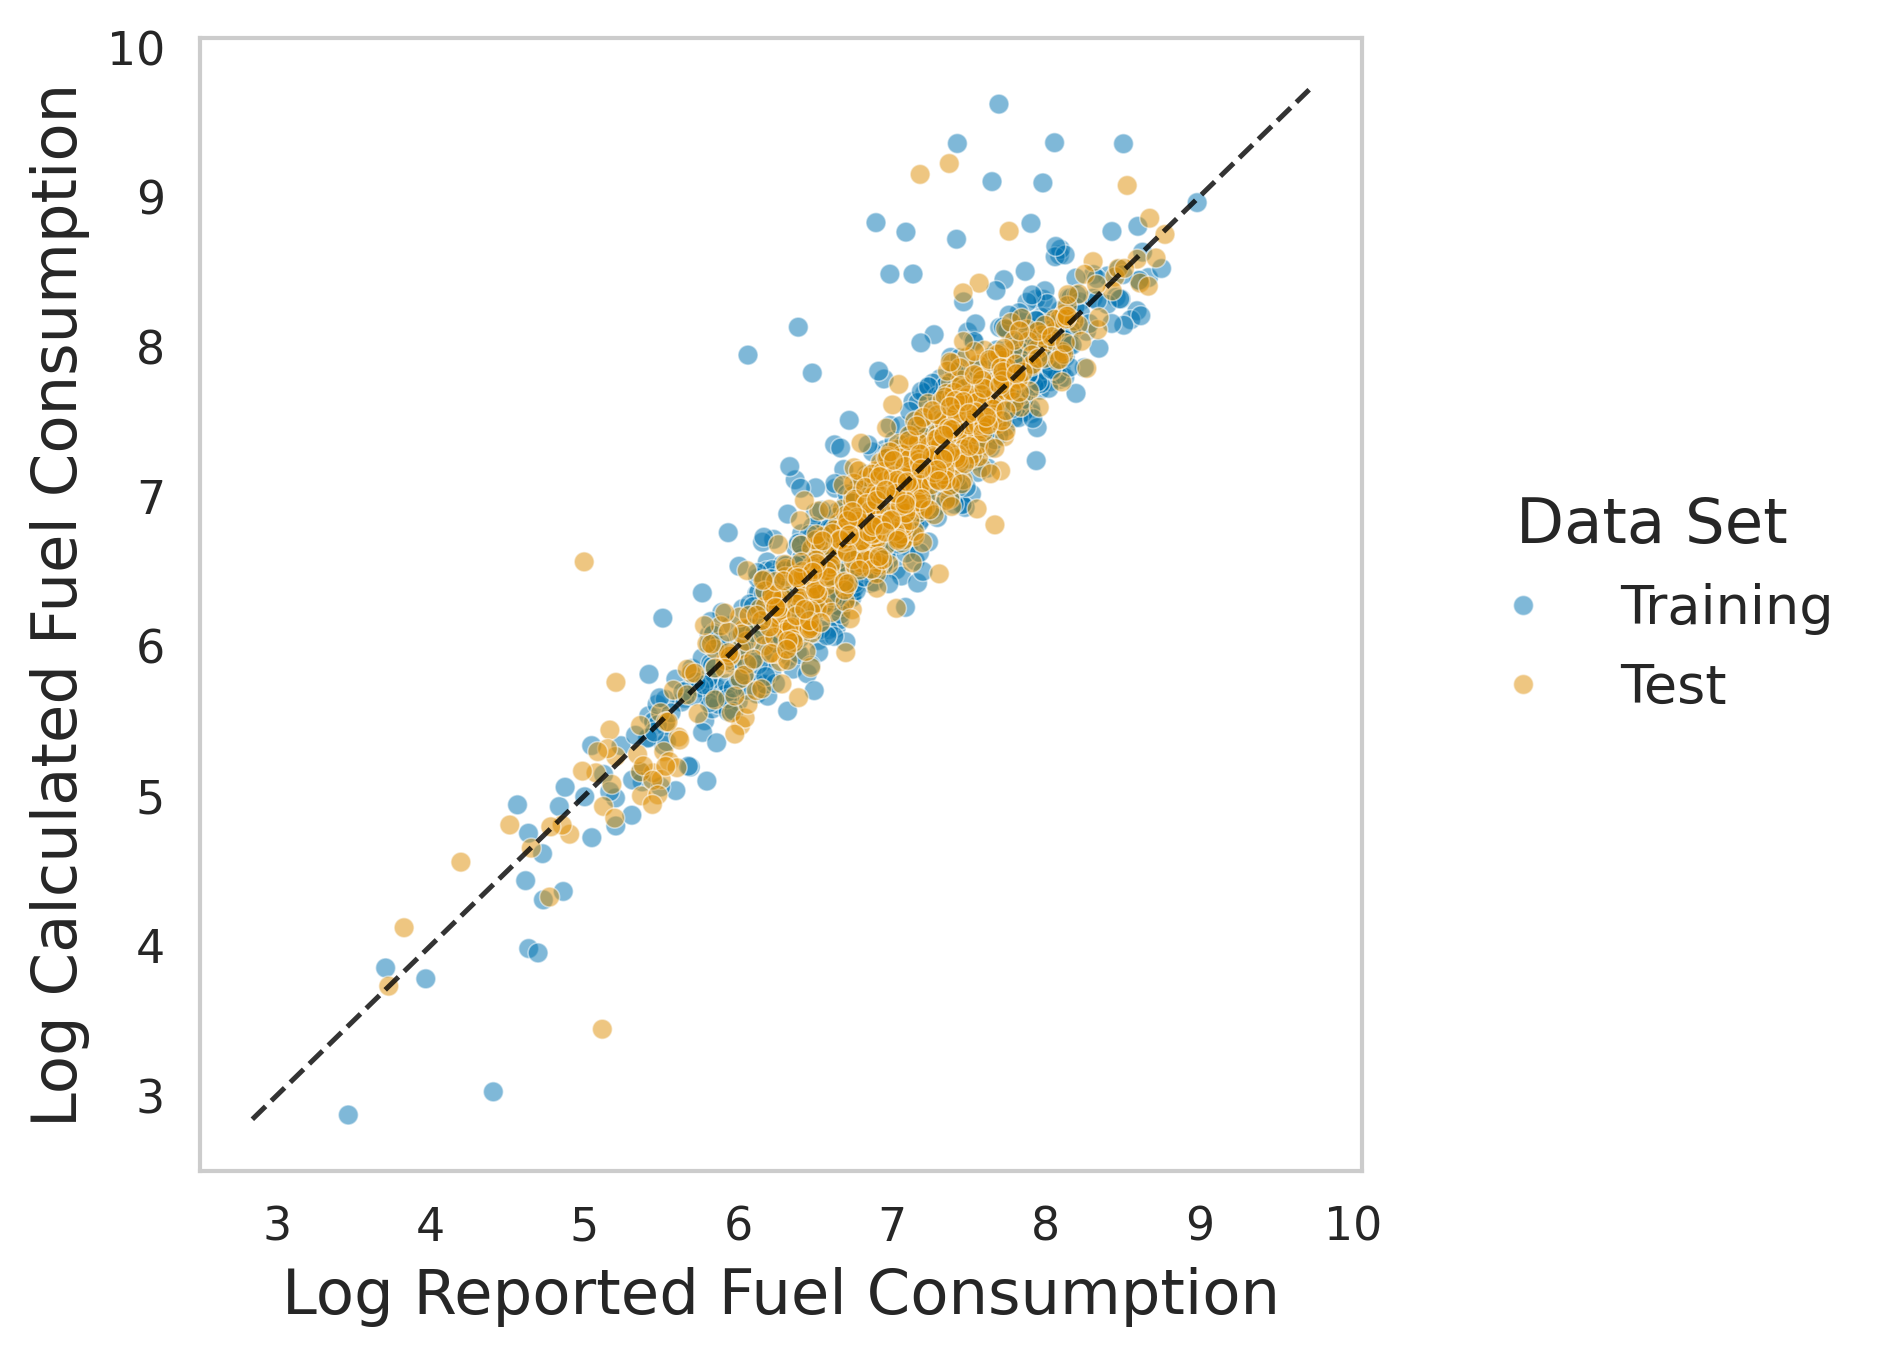
\includegraphics[width=0.65\textwidth]{ML_FC_Fm5dd_twoway_fc_filtered_traintest.png}
    \caption{Engineering calculations vs. reported fuel consumption}
    \label{fig:twoway_cal}
\end{figure}

% Tuning
The cross-validation training set performance of each optimally-tuned model is summarized in \autoref{tab:trainscores}, and the optimal parameters are provided in \autoref{tab:trainparams} in \autoref{app:ML}. The linear estimators perform slightly better than the tree-based models, both in terms of better average accuracy and less variation. Within the linear models, performance is almost identical, despite the regularization parameter being equal to one for ridge regression.
The overall best performance is achieved with ridge regression, giving an \ac{R2} of 0.956 and an \ac{MAPE} of 9.8\%. 

% Training set evaluation
\begin{table}
    \centering
    \begin{adjustbox}{max width=\textwidth}
    \begin{threeparttable}
        \caption{Training set cross-validation scores}
        \label{tab:trainscores}
        
\begin{tabular}[t]{lrrrrrr}
\toprule
\multicolumn{1}{c}{ } & \multicolumn{2}{c}{R$^2$} & \multicolumn{2}{c}{MAE (t)} & \multicolumn{2}{c}{MAPE (\%)} \\
\cmidrule(l{3pt}r{3pt}){2-3} \cmidrule(l{3pt}r{3pt}){4-5} \cmidrule(l{3pt}r{3pt}){6-7}
\multicolumn{1}{c}{Model} & \multicolumn{1}{c}{mean} & \multicolumn{1}{c}{sd} & \multicolumn{1}{c}{mean} & \multicolumn{1}{c}{sd} & \multicolumn{1}{c}{mean} & \multicolumn{1}{c}{sd}\\
\midrule
Ridge Regression & 0.956 & 0.019 & 122 & 13 & 9.8 & 0.7\\
Linear Regression & 0.956 & 0.020 & 122 & 14 & 9.8 & 0.7\\
Lasso & 0.954 & 0.020 & 125 & 14 & 10.0 & 0.7\\
Gradient Boosting Regressor & 0.942 & 0.039 & 130 & 16 & 10.6 & 0.9\\
CatBoost Regressor & 0.939 & 0.053 & 127 & 17 & 10.3 & 0.9\\
Random Forest Regressor & 0.914 & 0.036 & 157 & 19 & 12.3 & 1.0\\
\bottomrule
\end{tabular}

        \begin{tablenotes}[flushleft]\small
            \item \textit{Note:} Statistics computed from three repetitions of 10-fold validation.
        \end{tablenotes}
    \end{threeparttable}
    \end{adjustbox}
\end{table}

The true out-of-sample validation on the test set of 2021 data is very similar, as shown in \autoref{tab:testscores}. The linear models again out-perform the tree-based models in general, with ridge regression again achieving the highest \ac{R2}, at 0.954, corresponding to a \ac{MAPE} of 10.9\%. Interestingly, CatBoost very narrowly achieves the best \ac{MAPE} at 10.8\%. For comparison, the predictions of these two models are shown in \autoref{fig:twoway_test_compare2}.\footnote{See \autoref{fig:twoway_test_compare2_levels} in \autoref{app:ML} for the plot in levels.} CatBoost appears to perform slightly worse at high fuel consumption values. All models perform substantially better than the calculation-based approach, which achieves an \ac{R2} of only 0.58. For robustness, we repeat our analyses with alternative criteria for inclusion in the data set, both doubling the distance discrepancy and applying a relative difference of 10\%. The results are qualitatively similar, with slightly lower predictive accuracy with noisier data.\footnote{See Appendix \ref{app:altcriteria} for detailed results.}
% TODO: do these robustness checks and add to appendix

% Test set eval.
\begin{table}
    \centering
    \begin{adjustbox}{max width=\textwidth}
    \begin{threeparttable}
        \caption{Test set scores}
        \label{tab:testscores}
        
\begin{tabular}[t]{lrrr}
\toprule
\multicolumn{1}{c}{Model} & \multicolumn{1}{c}{R$^2$} & \multicolumn{1}{c}{MAE (t)} & \multicolumn{1}{c}{MAPE (\%)}\\
\midrule
Ridge Regression & 0.954 & 131 & 10.9\\
Linear Regression & 0.953 & 132 & 10.9\\
Lasso & 0.951 & 132 & 10.9\\
CatBoost Regressor & 0.941 & 133 & 10.8\\
Gradient Boosting Regressor & 0.939 & 143 & 11.6\\
Random Forest Regressor & 0.931 & 151 & 12.3\\
Calculation & 0.580 & 260 & 20.4\\
\bottomrule
\end{tabular}

        % \begin{tablenotes}[flushleft]\small
            % \item \textit{Note:} MAE is mean absolute error, and $R^2$ is the coefficient of determination. The best score for each metric is highlighted in bold.
        % \end{tablenotes}
    \end{threeparttable}
    \end{adjustbox}
\end{table}


\begin{figure}
    \centering
    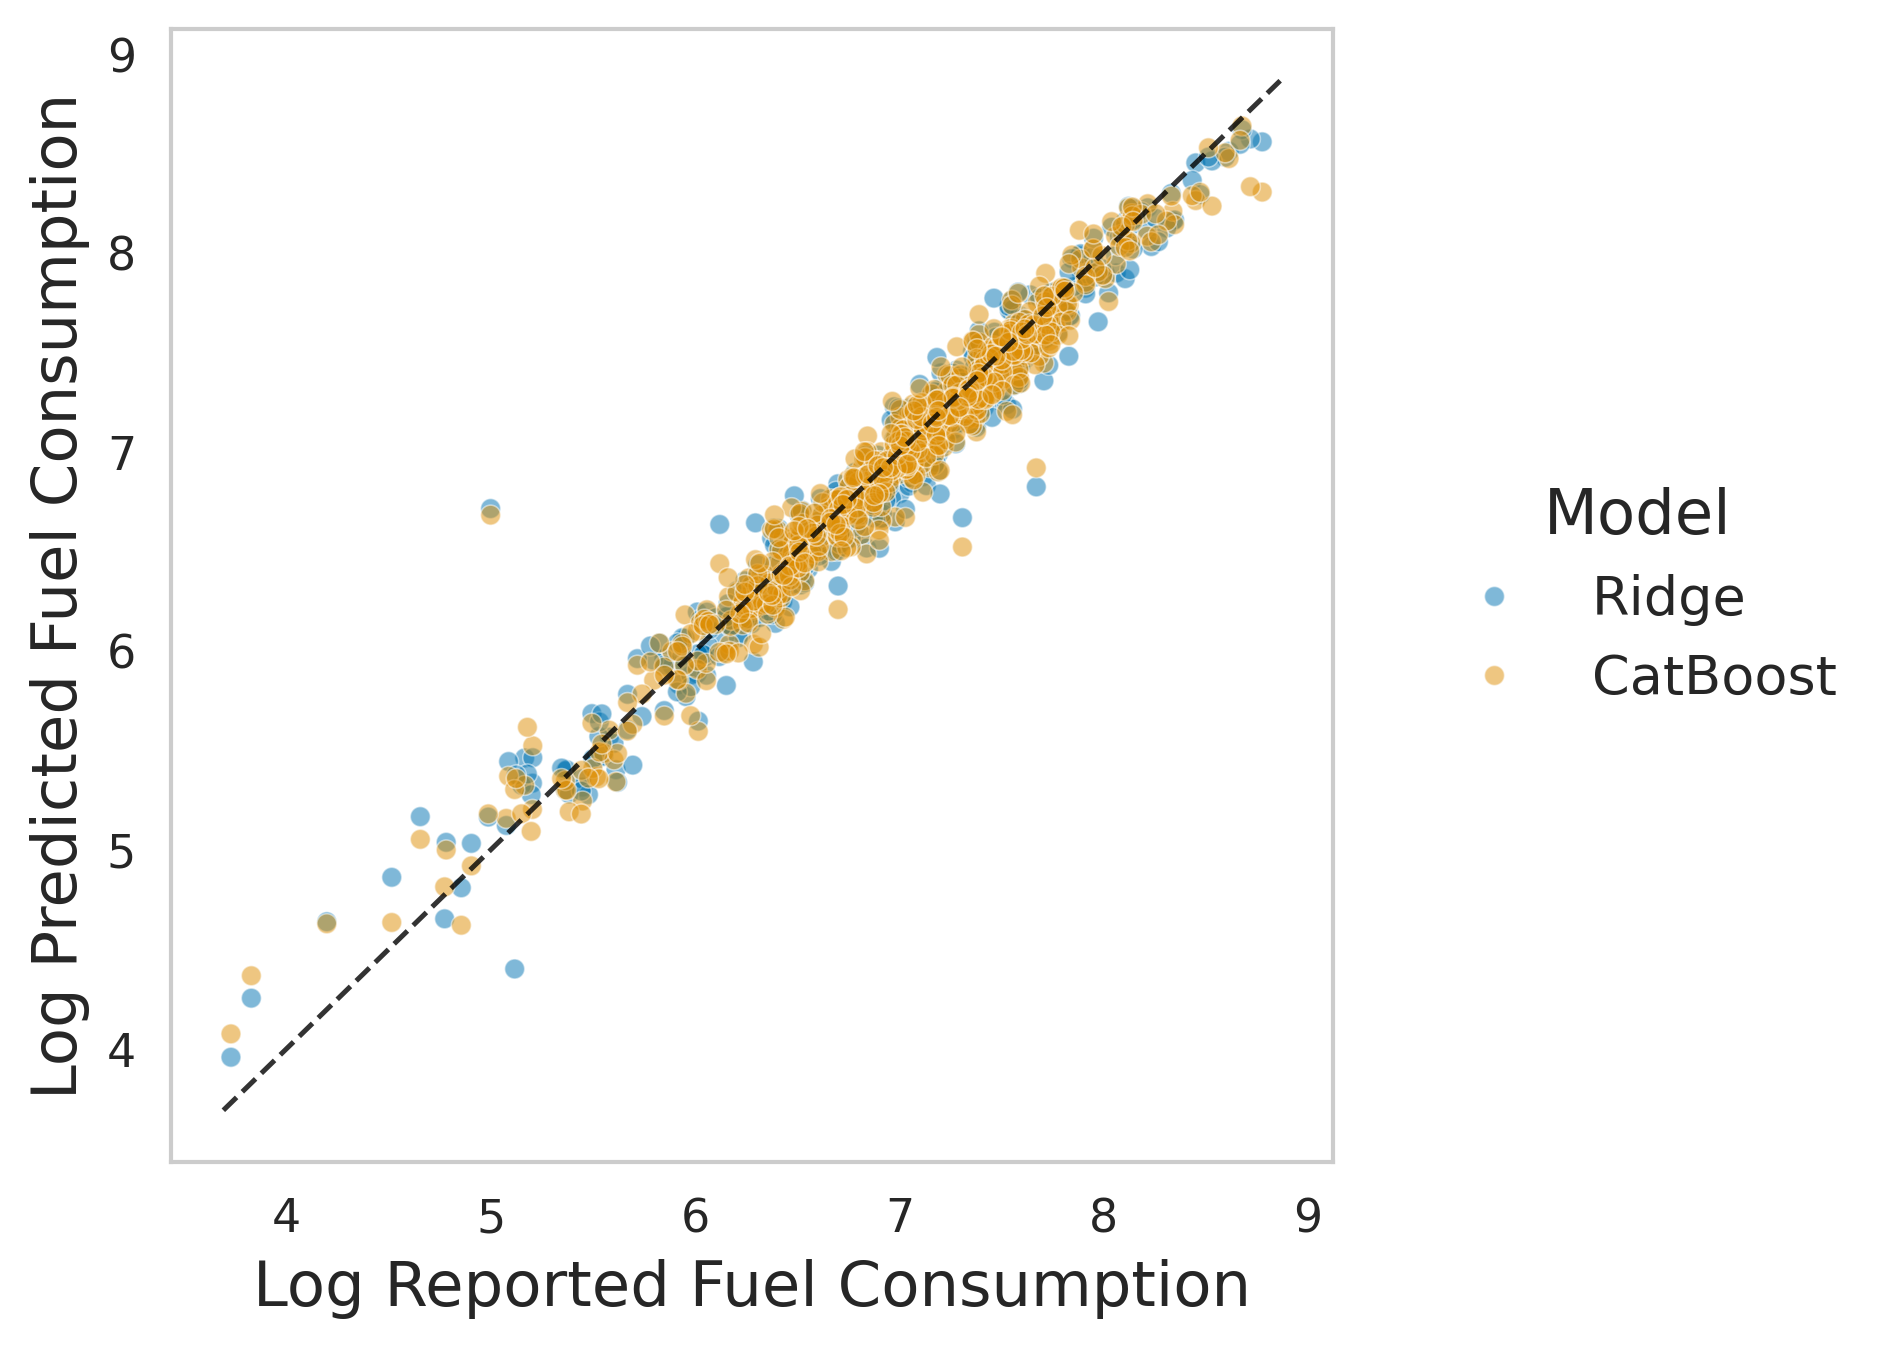
\includegraphics[width=0.65\textwidth]{ML_FC_Fm5dd_twoway_test_logs_compare2.png}
    \caption{Test set prediction accuracy (log-log) for ridge regression and CatBoost}
    \label{fig:twoway_test_compare2}
\end{figure}

% TODO: Discuss error-handling capacity of estimation over calculation

% TODO: Linear vs. non-linear models
% Why do some models work better than others?
% discuss log-additive discrepancy
% use feature importance to explain this
% is taking logs why linear models work so well?

% TODO: Feature importance
% TODO: dicuss utility of error variables and others
% for best? doesn't account for collinearity
% by groups? just run different subsets?

% Robustness
% - different feature sets?
\section{Conclusion}
Accurate and timely estimates of fuel consumption are key to understanding the drivers of \ac{GHG} emissions from maritime shipping and to assess the effectiveness of emissions policies. In this paper we have developed a highly accurate methodology for predicting \ac{CO2} emissions from readily-available tracking ship tracking data, which can be employed at an arbitrary frequency or with any subset of ships that may be of interest. To carefully capture the nonlinear effects of travel speed, we take a hybrid approach in which we calculate predictor variables from industry-standard fuel consumption formulas. We demonstrate a substantial increase in predictive accuracy over the pure calculation-based approach. Our results are not particularly sensitive to the specific machine learning model that is employed, and in fact computationally-efficient linear models perform best. It is our hope that this approach will be employed to provide more accurate and up-to-date estimates of shipping emissions.



% 


\appendix
\section{Data Cleaning}\label{app:MLDataCleaning}

% number of missing obs?

% no invalid long, lat values
% no speed values above 30 knots (according t Oliver)
% implied speed?
% Source: AIS_Calculations.py

% Jumps
% greater than 170 above 5 knots or 
% Source: AIS_Calculations.py

% number of impossible values?
% number of jumps?
% number of drafts infilled?

% After interpolation
% high speed values!
% high distance values

\section{Summary Statistics}\label{app:summarystats}

% representativeness of EU MRV reporting fleet
% mean, sd of all variables

\section{Trip Detection}\label{app:tripdetection}


\section{Machine Learning Details}\label{app:mldetails}

The optimal tuning parameters are provided in \autoref{tab:trainparams}.
\begin{table}[H]
    \centering
    \begin{adjustbox}{max width=\textwidth}
    \begin{threeparttable}
        \caption{Optimal tuning parameters}
        \label{tab:trainparams}
        
\begin{tabular}[t]{llr}
\toprule
\multicolumn{1}{l}{Model} & \multicolumn{1}{l}{Parameter} & \multicolumn{1}{l}{Value}\\
\midrule
 & depth & 6\\

 & l2 leaf reg & 1\\

\multirow[t]{-3}{*}{\raggedright\arraybackslash CatBoost Regressor} & learning rate & 0.1\\
\cmidrule(lr){1-3}

 & learning rate & 0.01\\

\multirow[t]{-2}{*}{\raggedright\arraybackslash Gradient Boosting Regressor} & max depth & 3\\
\cmidrule(lr){1-3}

Lasso & alpha & 0.005\\
\cmidrule(lr){1-3}

Linear Regression & n/a & n/a\\
\cmidrule(lr){1-3}

 & max depth & 50\\

\multirow[t]{-2}{*}{\raggedright\arraybackslash Random Forest Regressor} & n estimators & 200\\
\cmidrule(lr){1-3}

Ridge Regression & alpha & 10\\
\bottomrule
\end{tabular}

        % \begin{tablenotes}[flushleft]\small
            % \item \textit{Note:} MAE is mean absolute error, and $R^2$ is the coefficient of determination. The best score for each metric is highlighted in bold.
        % \end{tablenotes}
    \end{threeparttable}
    \end{adjustbox}
\end{table}

The inferior performance of the CatBoost model versus ridge regression is shown in \autoref{fig:twoway_test_compare2_levels}.
\begin{figure}[H]
    \centering
    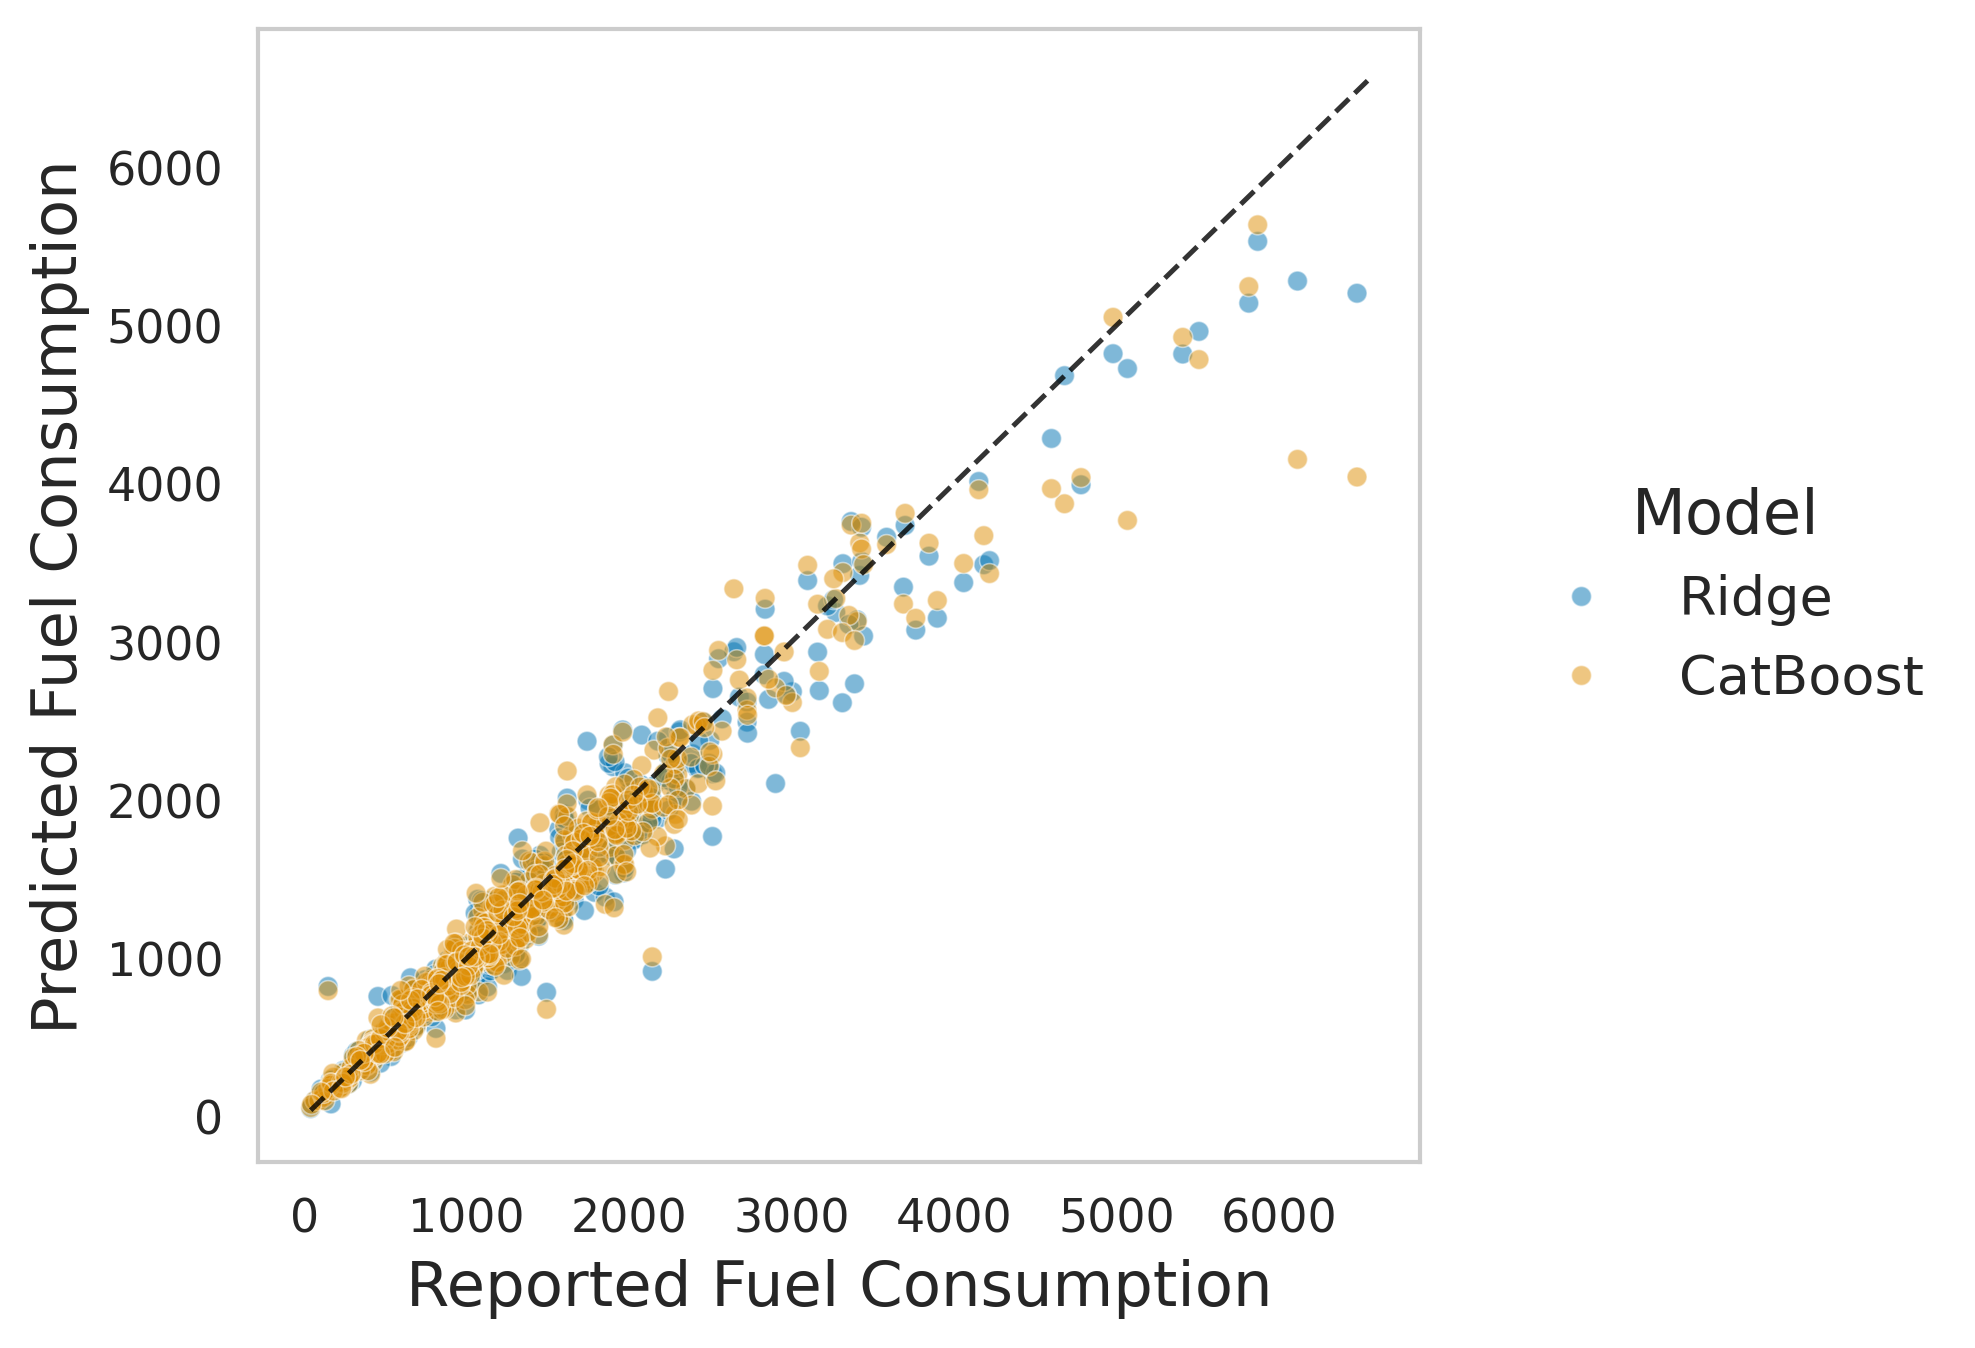
\includegraphics[width=0.65\textwidth]{ML_FC_Fm5dd_twoway_test_levels_compare2.png}
    \caption{Test set prediction accuracy (levels) for ridge regression and CatBoost}
    \label{fig:twoway_test_compare2_levels}
\end{figure}

\section{Alternative Data Inclusion Criteria}\label{app:altcriteria}

\end{document}